% !TeX spellcheck = en_US
\newpage
\section{Reproducibility}
Most computer based experiments are \textbf{repeatable} while the result of an experiment is \textbf{reproducible} if it's not affected substantially by a limited perturbation of the setup.
\begin{center}
	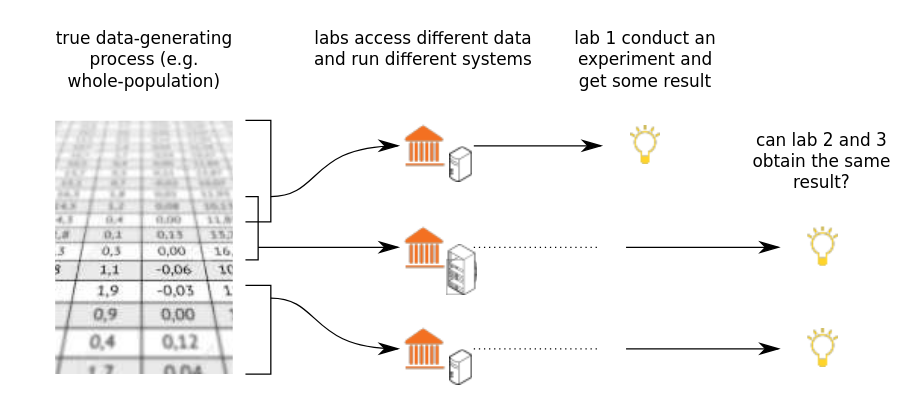
\includegraphics[scale=.4]{reprod}
\end{center}

\subsection{Testing}
\subsubsection{Holdout}
\begin{wrapfigure}[6]{r}{7cm}
	\vspace{-1.3cm}
	\begin{center}
		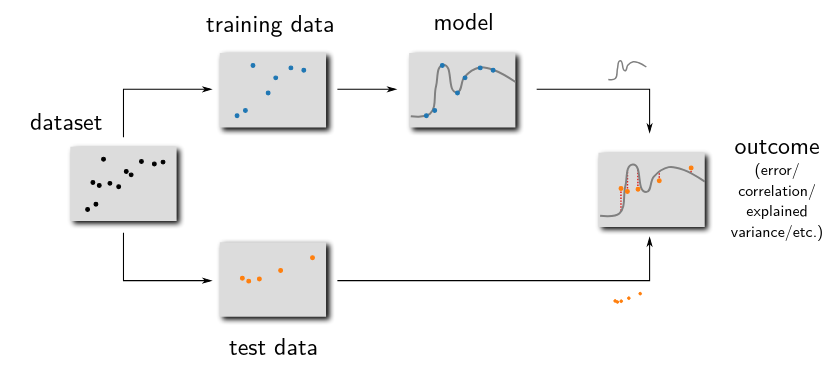
\includegraphics[width=7cm]{holdout}
	\end{center}
\end{wrapfigure}
The idea behind this procedure is to artificially simulate the scenario of another lab reproducing the experiment by randomly partitioning  the available data into \textbf{training} and \textbf{test}. The learning is done on the training data  and the report and results on the test one.

\begin{example}[PCA]
	In the PCA we learn the first principal component $\mathbf{u}_1$ on the \textit{training} data:
	\begin{align*}
		& C_{\text{train}} = \text{Cov}(X_{\text{train}}, X_{\text{train}}) &\text{(estimate the covariance)}\\
		& \mathbf{u}_1 = \arg\max_\mathbf{u} \mathbf{u}^\top C_\text{train} \mathbf{u} & \text{(extract the PCA-1 direction)}
	\end{align*}
	And then we measure the variance explained by $\mathbf{u}_1$ on the \textit{test} data:
	\begin{align*}
		& C_\text{test} = \text{Cov}(X_\text{test}, X_\text{test}) & \text{(estimate the covariance)} \\
		& \lambda_\text{test} = \mathbf{u}_1^\top C_\text{test} \mathbf{u}_1 & \text{(compute the explained variance)}
	\end{align*}
\end{example}

\begin{example}[Least Square Regression]
	In Least Square Regression we train the regression model on the \textit{training} data:
	\begin{align*}
		& C_{xx} = \text{Cov}(X_\text{train}, X_\text{train}) & \text{(estimate the auto-covariance)} \\
		& C_{xy} = \text{Cov}(X_\text{train}, Y_\text{train}) & \text{(estimate the cross-covariance)} \\
		& \mathbf{w} = C^{-1}_{xx}C_{xy} \\
		&b = \mathbb{E}[Y_\text{train}] - \mathbf{w}^\top \mathbb{E}[X_\text{train}]
	\end{align*}
	And then we evaluate the error of the model $(\mathbf{w}, b)$ on the \textit{test} data:
	\begin{align*}
		& \hat{Y}_\text{test} = \mathbf{w}^\top X_\text{test} + b & \text{(predict the test data)} \\
		& \varepsilon_\text{test} = \mathbb{E}[(\hat{Y}_\text{test}-Y_\text{test})^2] & \text{(compute the prediction error)}
	\end{align*}
\end{example}

\newpage
\subsubsection{Cross-Validation}
\begin{wrapfigure}[7]{r}{7cm}
	\vspace{-.9cm}
	\begin{center}
		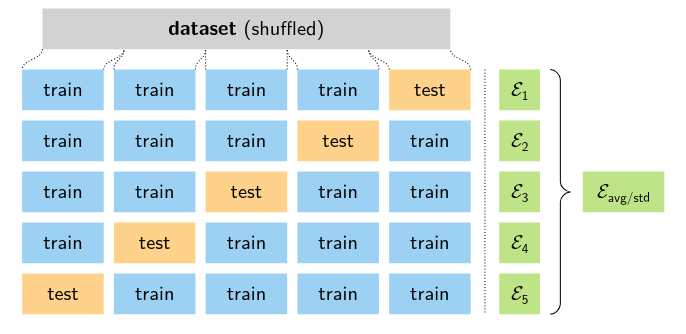
\includegraphics[width=7cm]{crossval}
	\end{center}
\end{wrapfigure}
If by splitting data evenly into a training and test set there is not much data left for both procedures, we get worse models and noisier error estimates. This can be addressed by cross-validation: repeating the analysis over \textbf{multiple splits} and \textbf{averaging} the results. Since this operation reduces the noise of error estimates, most of data should be allocated fro training ($80\%$).

\paragraph{Overfitting} This phenomena causes models that perform better on the training set to do worse on the test one. This is due to the model trying to extract more variations that can possibly be recovered from the input features, lowering the training error but performing worse on out-of-sample data.
\begin{center}
	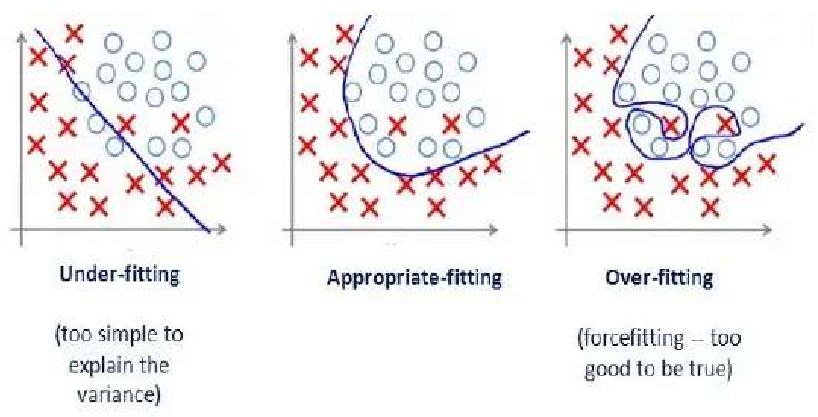
\includegraphics[scale=.4]{overfit}
\end{center}

\subsection{Modeling complexity}
\begin{wrapfigure}[7]{r}{6cm}
	\vspace{-.9cm}
	\begin{center}
		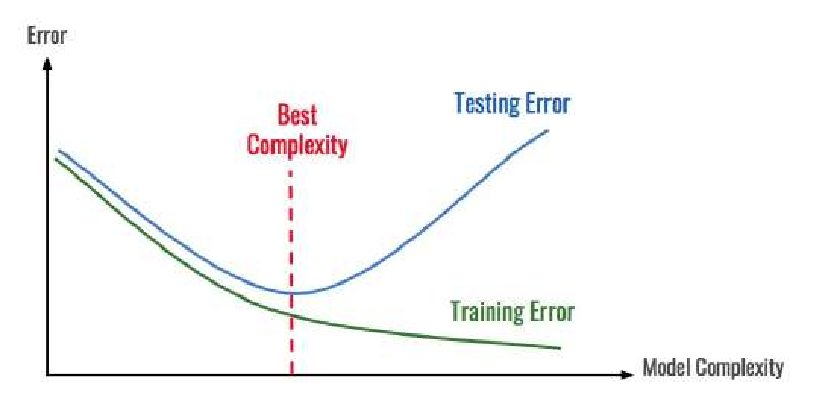
\includegraphics[width=6cm]{modelcomp}
	\end{center}
\end{wrapfigure}
By controlling the complexity of a model, one can reach a good trade off between \textbf{underfitting} and \textbf{overfitting}, hence performing better on the test data.\\

To do this we need a mechanism within the learning procedure to control model complexity so that we can adjust it. There are two approaches:
\begin{itemize}
	\item \textbf{Feature selection}: define a limited set of features $\mathcal{I}$, with $\lvert\mathcal{I}\rvert < d$, that the model can use for training
	\item \textbf{Model regularization}: penalize models that are oversensitive to small variations of the data, e.g. for a linear model impose $\lvert\lvert \mathbf{w}\rvert\rvert^2 < R$ on the weight. The lower the \textit{hyperparameter} R, the less likely to overfit
\end{itemize}

\subsubsection{Least Square Regression}
To regularize LSR we proceed in two steps:
\begin{enumerate}
	\item Build the Lagrangian
	\begin{equation*}
		\mathcal{L}(\mathbf{w}, \lambda) = \frac{1}{2} \mathbb{E}[\lvert\lvert\mathbf{w}^\top\mathbf{x}-y\rvert\rvert^2] + \frac{1}{2}\lambda(\lvert\lvert \mathbf{w} \rvert\rvert^2-S)
	\end{equation*}
	\newpage
	\item Verify Slater's conditions and apply the KKT conditions:
	\begin{itemize}
		\item \textbf{Stationarity} gives us:
		\begin{equation*}
			\frac{\nabla\mathcal{L}}{\nabla\mathbf{w}} = \underbrace{\mathbb{E}[\mathbf{x}\mathbf{x}^\top]}_{C_{xx}}\mathbf{w} - \underbrace{\mathbb{E}[\mathbf{x}y]}_{C_{xy}} + \lambda\mathbf{w} \overset{\text{def}}{=} \mathbf{0}
		\end{equation*}
		and therefore
		\begin{equation*}
			\mathbf{w} = (C_{xx}+\lambda I)^{-1}C_{xy}
		\end{equation*}
		\item \textbf{Complementary slackness} gives us:
		\begin{equation*}
			\lambda \cdot (\lvert\lvert \mathbf{w}\rvert\rvert^2 - S) = 0
		\end{equation*}
		If $\lambda > 0$ then $\lvert\lvert \mathbf{w}\rvert\rvert^2=S$. If $\lvert\lvert \mathbf{w}\rvert\rvert^2<S$ then $\lambda=0$ (standard regression).
	\end{itemize}
\end{enumerate}

\begin{center}
	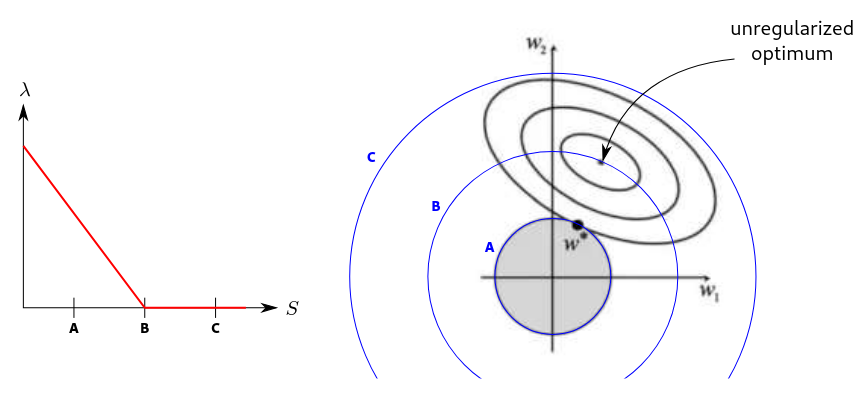
\includegraphics[scale=.4]{reglsr}
\end{center}

\begin{observation}
	Since we want to try many parameter $S$, we should not try to resolve $\lambda$ from it but instead try different parameters $\lambda$ too.
\end{observation}

\subsubsection{Fisher Discriminant}
Like with the Least Square Regression, the Fisher discriminant can be expressed with regularization as:
\begin{equation*}
	\mathbf{w} = (C_{xx}+\lambda I)^{-1}(\mu_2 - \mu_1)
\end{equation*}
Increasing $\lambda$ makes the inverse covariance term more similar to an identity and the direction $\mathbf{w}$ becomes aligned with that of the difference of means ($\mathbf{w} = \mu_2-\mu_1$).
\begin{center}
	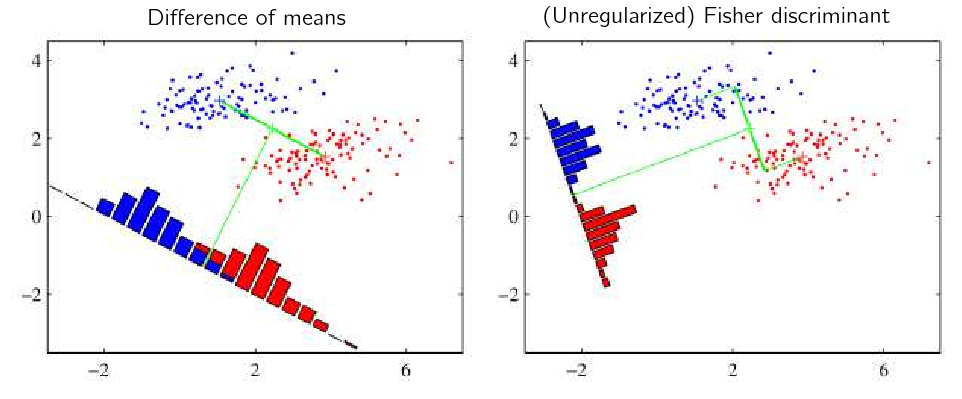
\includegraphics[scale=.4]{fisherreg}
\end{center}

\subsection{Vapnik-Chervonenkis Theory}
Now we want to formally connect model complexity to the true (\textit{reproducible}) error of a model.\\

We can define the true error, given a ground-truth joint distribution $p(\mathbf{x},y)$ over the input $\mathbf{x} \in \mathbb{R}^d$ and the output $y \in \mathbb{R}^d$, of some predictor $f: \mathbb{R}^d \to \mathbb{R}$ by the integral:
\begin{equation}
	\varepsilon_\text{true}(f) = \int \ell(f(\mathbf{x}),y)dp(\mathbf{x},y)
\end{equation}
where $\ell(f(\mathbf{x}),y)$ is some \textbf{loss function}. In practice $p$ is unknown and therefore we only know the \textit{train} error:
\begin{equation}
	\varepsilon_\text{train}(f) = \frac{1}{N} \sum_{i=1}^{N}\ell(f(\mathbf{x}_i), y_i)
\end{equation}

Vapnik-Chervonenkis theory provide a connection between training and true error in the context of classification. Specifically, it shows that with probability $1 - \delta$:
\begin{equation}
	\varepsilon_\text{true}(f) - \varepsilon_\text{train}(f) \leq \sqrt{\frac{h_\mathcal{F} \cdot \bigg(\log\bigg(\frac{2N}{h_\mathcal{F}}\bigg)+1\bigg)-\log\bigg(\frac{\delta}{4}\bigg)}{N}}
\end{equation}
where $h_\mathcal{F}$ is the VC \textbf{dimension} measuring the complexity of the class models $\mathcal{F}$ which ours is selected from. Specifically, the maximum number of data points that the class can always classify in any possible way. Some examples are:
\begin{itemize}
	\item $
		f(\mathbf{x}) = \text{sign}(\sin(\mathbf{w}^\top \mathbf{x}+b)) \qquad\qquad\qquad\qquad h_\mathcal{F} = \infty
$
	\item $
		f(\mathbf{x}) = \text{sign}(\mathbf{w}^\top \mathbf{x}+b) \qquad\qquad\qquad\qquad\qquad h_\mathcal{F} = d+1
$
	\item $
		f(\mathbf{x}) = \text{sign}(\mathbf{w}^\top \mathbf{x}+b)\qquad \frac{1}{\lvert\lvert \mathbf{w} \rvert\rvert} = \frac{M}{2} \qquad\qquad h_\mathcal{F} \leq \min\{d+1, \lceil \frac{4r^2}{M^2} \rceil +1\}
$
\end{itemize}